\documentclass{beamer}

%%%%%%%%%%%%%Solarized Theme%%%%%%%%%%%%%%%
\usecolortheme[dark,accent=cyan]{solarized}
\beamertemplatenavigationsymbolsempty
%%%%%Packages%%%%%
\usefonttheme{serif}
\usepackage[T1]{fontenc}
\usepackage[utf8]{inputenc}
\usepackage[english]{babel}
\usepackage{fontawesome}
\usepackage{minted}
\usepackage{soul}
\usepackage{ulem}
\usepackage{blkarray}
\usepackage{multirow}

\definecolor{DarkGray}{gray}{0.1}
\usemintedstyle{paraiso-dark}


\usepackage{graphicx}
\usepackage{hyperref}
\usepackage{colortbl, xcolor}
\usepackage{booktabs}
\usepackage{amsmath,amsthm, amssymb, latexsym}

\usepackage{tikz}
\usepackage{xcolor}
\usepackage{graphicx,multirow}
\definecolor{plain}{rgb}{93,93,93}
\usetikzlibrary{positioning,arrows}
\definecolor{applegreen}{rgb}{0.55, 0.71, 0.0}
\usetikzlibrary{decorations.pathreplacing, backgrounds, fit}
\usetikzlibrary{calc,matrix}

\tikzstyle{background}=[solarizedRed, rectangle, draw, inner sep=1mm, thick,
           rounded corners=2mm]

\tikzset{
  treenode/.style = {align=center, inner sep=0pt, text centered,
    font=\sffamily},
  arn_n/.style = {treenode, circle, white, font=\sffamily\bfseries, draw=black, inner sep=-6pt,
    fill=black, text width=1.5em},% arbre rouge noir, noeud noir
  arn_r/.style = {treenode, circle, red, 
    text width=1.5em, very thick, inner sep=4pt},% arbre rouge noir, noeud rouge
  arn_x/.style = {treenode, rectangle, draw=black,
    minimum width=0.5em, minimum height=0.5em}% arbre rouge noir, nil
}

\usepackage{standalone}
\usepackage{siunitx}

\begin{document}

\begin{frame}
    \begin{center}
        \Large{\textcolor{orange}{Evolution of cooperation among individuals with limited payoff memory}} \\
        \vspace{.5cm}
        \large{AQUAVIT}

        \vspace{1cm}
        \normalsize{@NikoletaGlyn} \\
        \vspace{.5cm}
        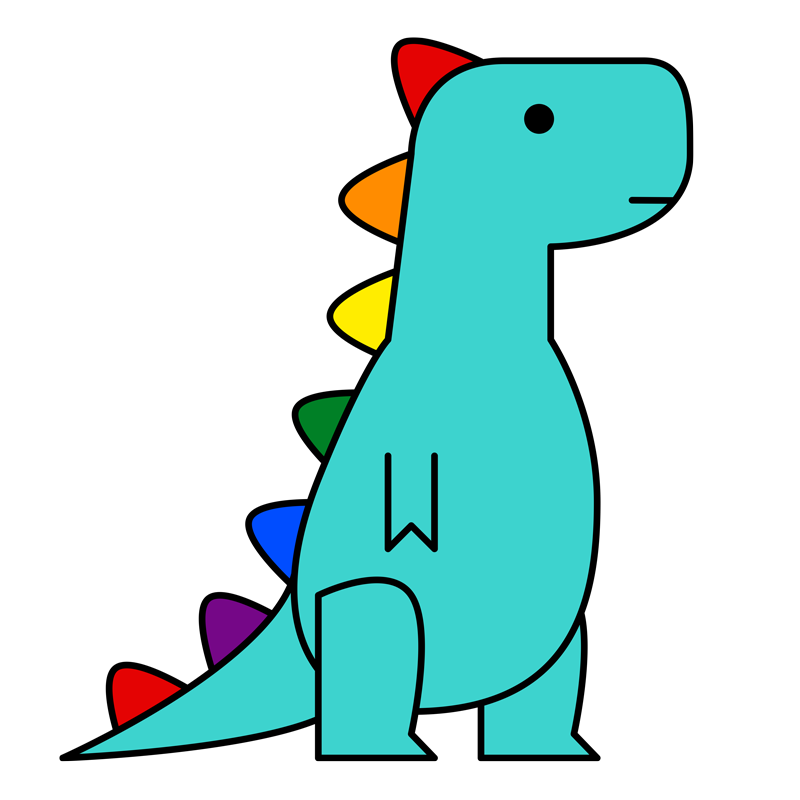
\includegraphics[width=0.14\textwidth]{static/dyno.png}

    \end{center}
\end{frame}

\begin{frame}
    \begin{center}
    
\includegraphics[width=0.24\textwidth]{static/mpi.jpg}\hspace{8pt}
    
\includegraphics[width=0.24\textwidth]{static/cardiff_uni_logo.jpg}\vspace{8pt}

    
\includegraphics[width=0.24\textwidth]{static/ssi-logo.png}\hspace{8pt}
    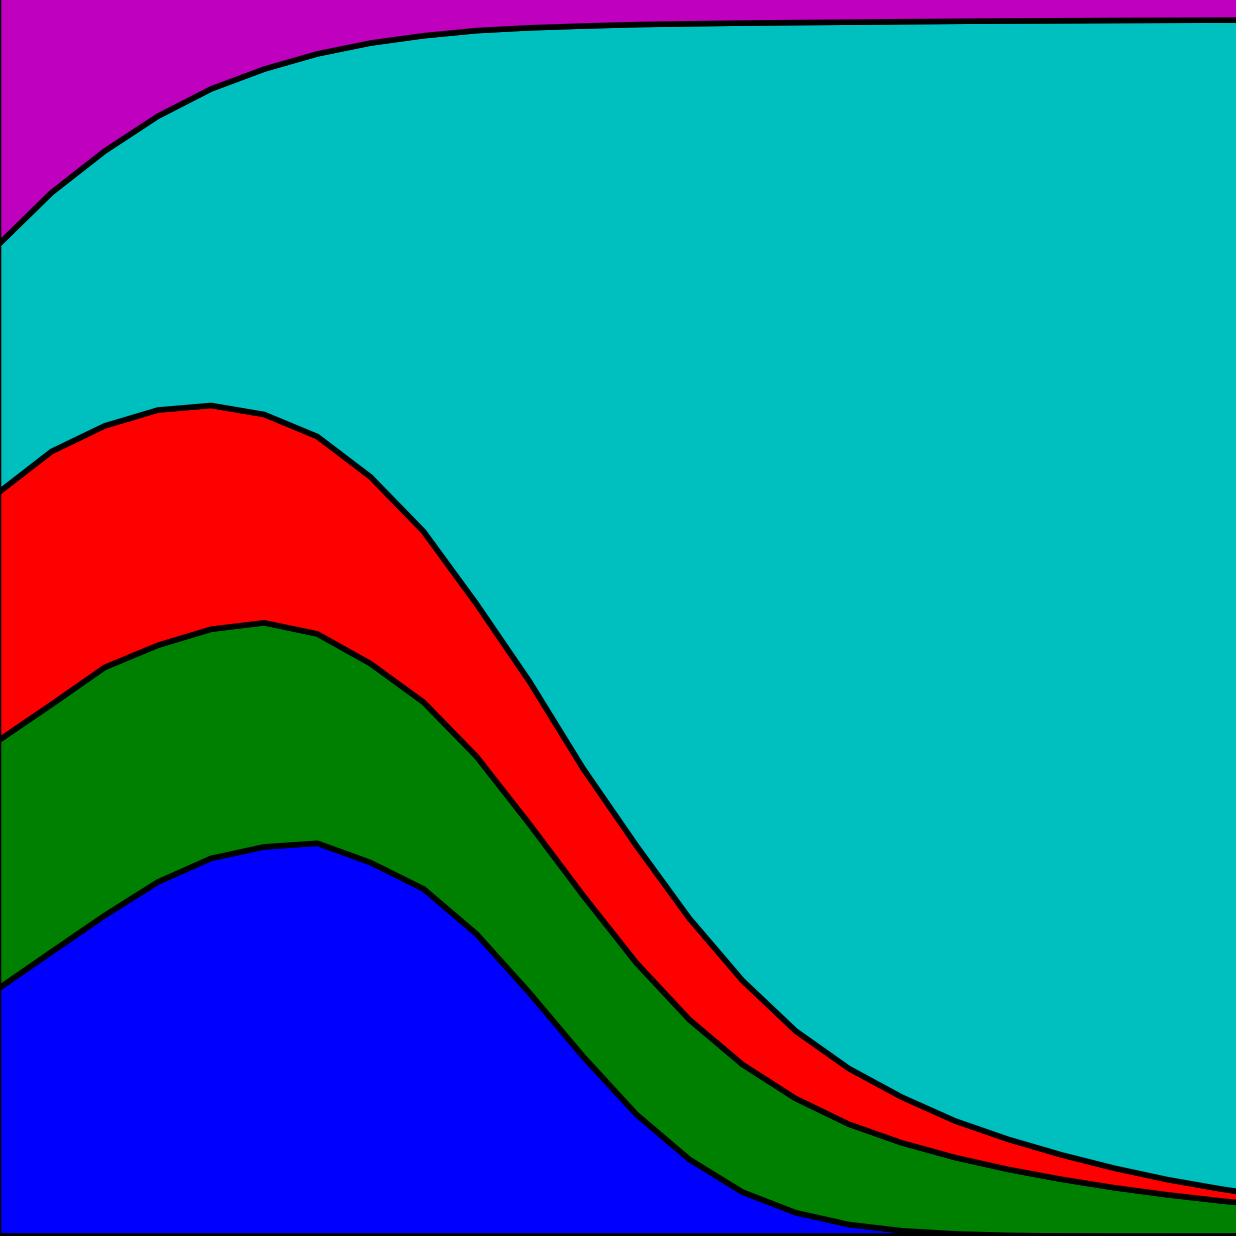
\includegraphics[width=0.24\textwidth]{static/axelrod-logo.png}
    \end{center}
\end{frame}

\begin{frame}
    \centering
    \includestandalone[width=.75\textwidth]{static/game}
\end{frame}


\begin{frame} \textbf{
    \begin{center}
    \LARGE{
        \begin{equation*}
            \begin{blockarray}{ccc}
               & \text{\textcolor{cyan}{Nice}} & \text{\textcolor{orange}{Not Nice}} \\
                \begin{block}{c(cc)}
                \text{\textcolor{cyan}{Nice} } & (b - c, b - c) & (-c, b) \\
                \text{\textcolor{orange}{Not Nice} } & (b, -c) & (0, 0) \\
                \end{block}
            \end{blockarray}
        \end{equation*}}
    \end{center}}
\end{frame}

\begin{frame} \textbf{
    \begin{center}
    \LARGE{
        \begin{equation*}
            \begin{blockarray}{ccc}
               & \text{\textcolor{cyan}{Nice}} & \text{\textcolor{orange}{Not Nice}} \\
                \begin{block}{c(cc)}
                \text{\textcolor{cyan}{Nice} } & (2, \phantom{-}2) & (-1, 3) \\
                \text{\textcolor{orange}{Not Nice} } & (3, -1) & (\phantom{-}0, 0) \\
                \end{block}
            \end{blockarray}
        \end{equation*}}
    \end{center}}
\end{frame}

\begin{frame}
    \begin{center}
\includestandalone[width=\textwidth]{static/iterated_prisoners_dilemma}
    \end{center}
\end{frame}

\begin{frame}
    \centering
    \includestandalone[width=.65\textwidth]{static/population}
\end{frame}

\begin{frame}
    \centering
    \includestandalone[width=.65\textwidth]{static/population_c}
\end{frame}

\begin{frame}
    \centering
    \includestandalone[width=.65\textwidth]{static/population_d}
\end{frame}

\begin{frame}
    \centering
    \includestandalone[width=.65\textwidth]{static/reactive}
\end{frame}

\begin{frame}
    \begin{columns}
        \begin{column}[]{.55\textwidth}
            \centering
            \includestandalone[width=.67\textwidth]{static/game_stage}
        \end{column}
        \begin{column}[]{.45\textwidth}
            \includestandalone[width=.82\textwidth]{static/evolution}
        \end{column}
    \end{columns}
\end{frame}

\begin{frame}
    \centering
    \includestandalone[width=.75\textwidth]{static/fitness}
\end{frame}

\begin{frame}
    \centering
    \includestandalone[width=.8\textwidth]{static/last_rounds_matches}
\end{frame}

\begin{frame}
    \centering
    \includestandalone[width=\textwidth]{static/last_round}
\end{frame}

\begin{frame}
    \centering
    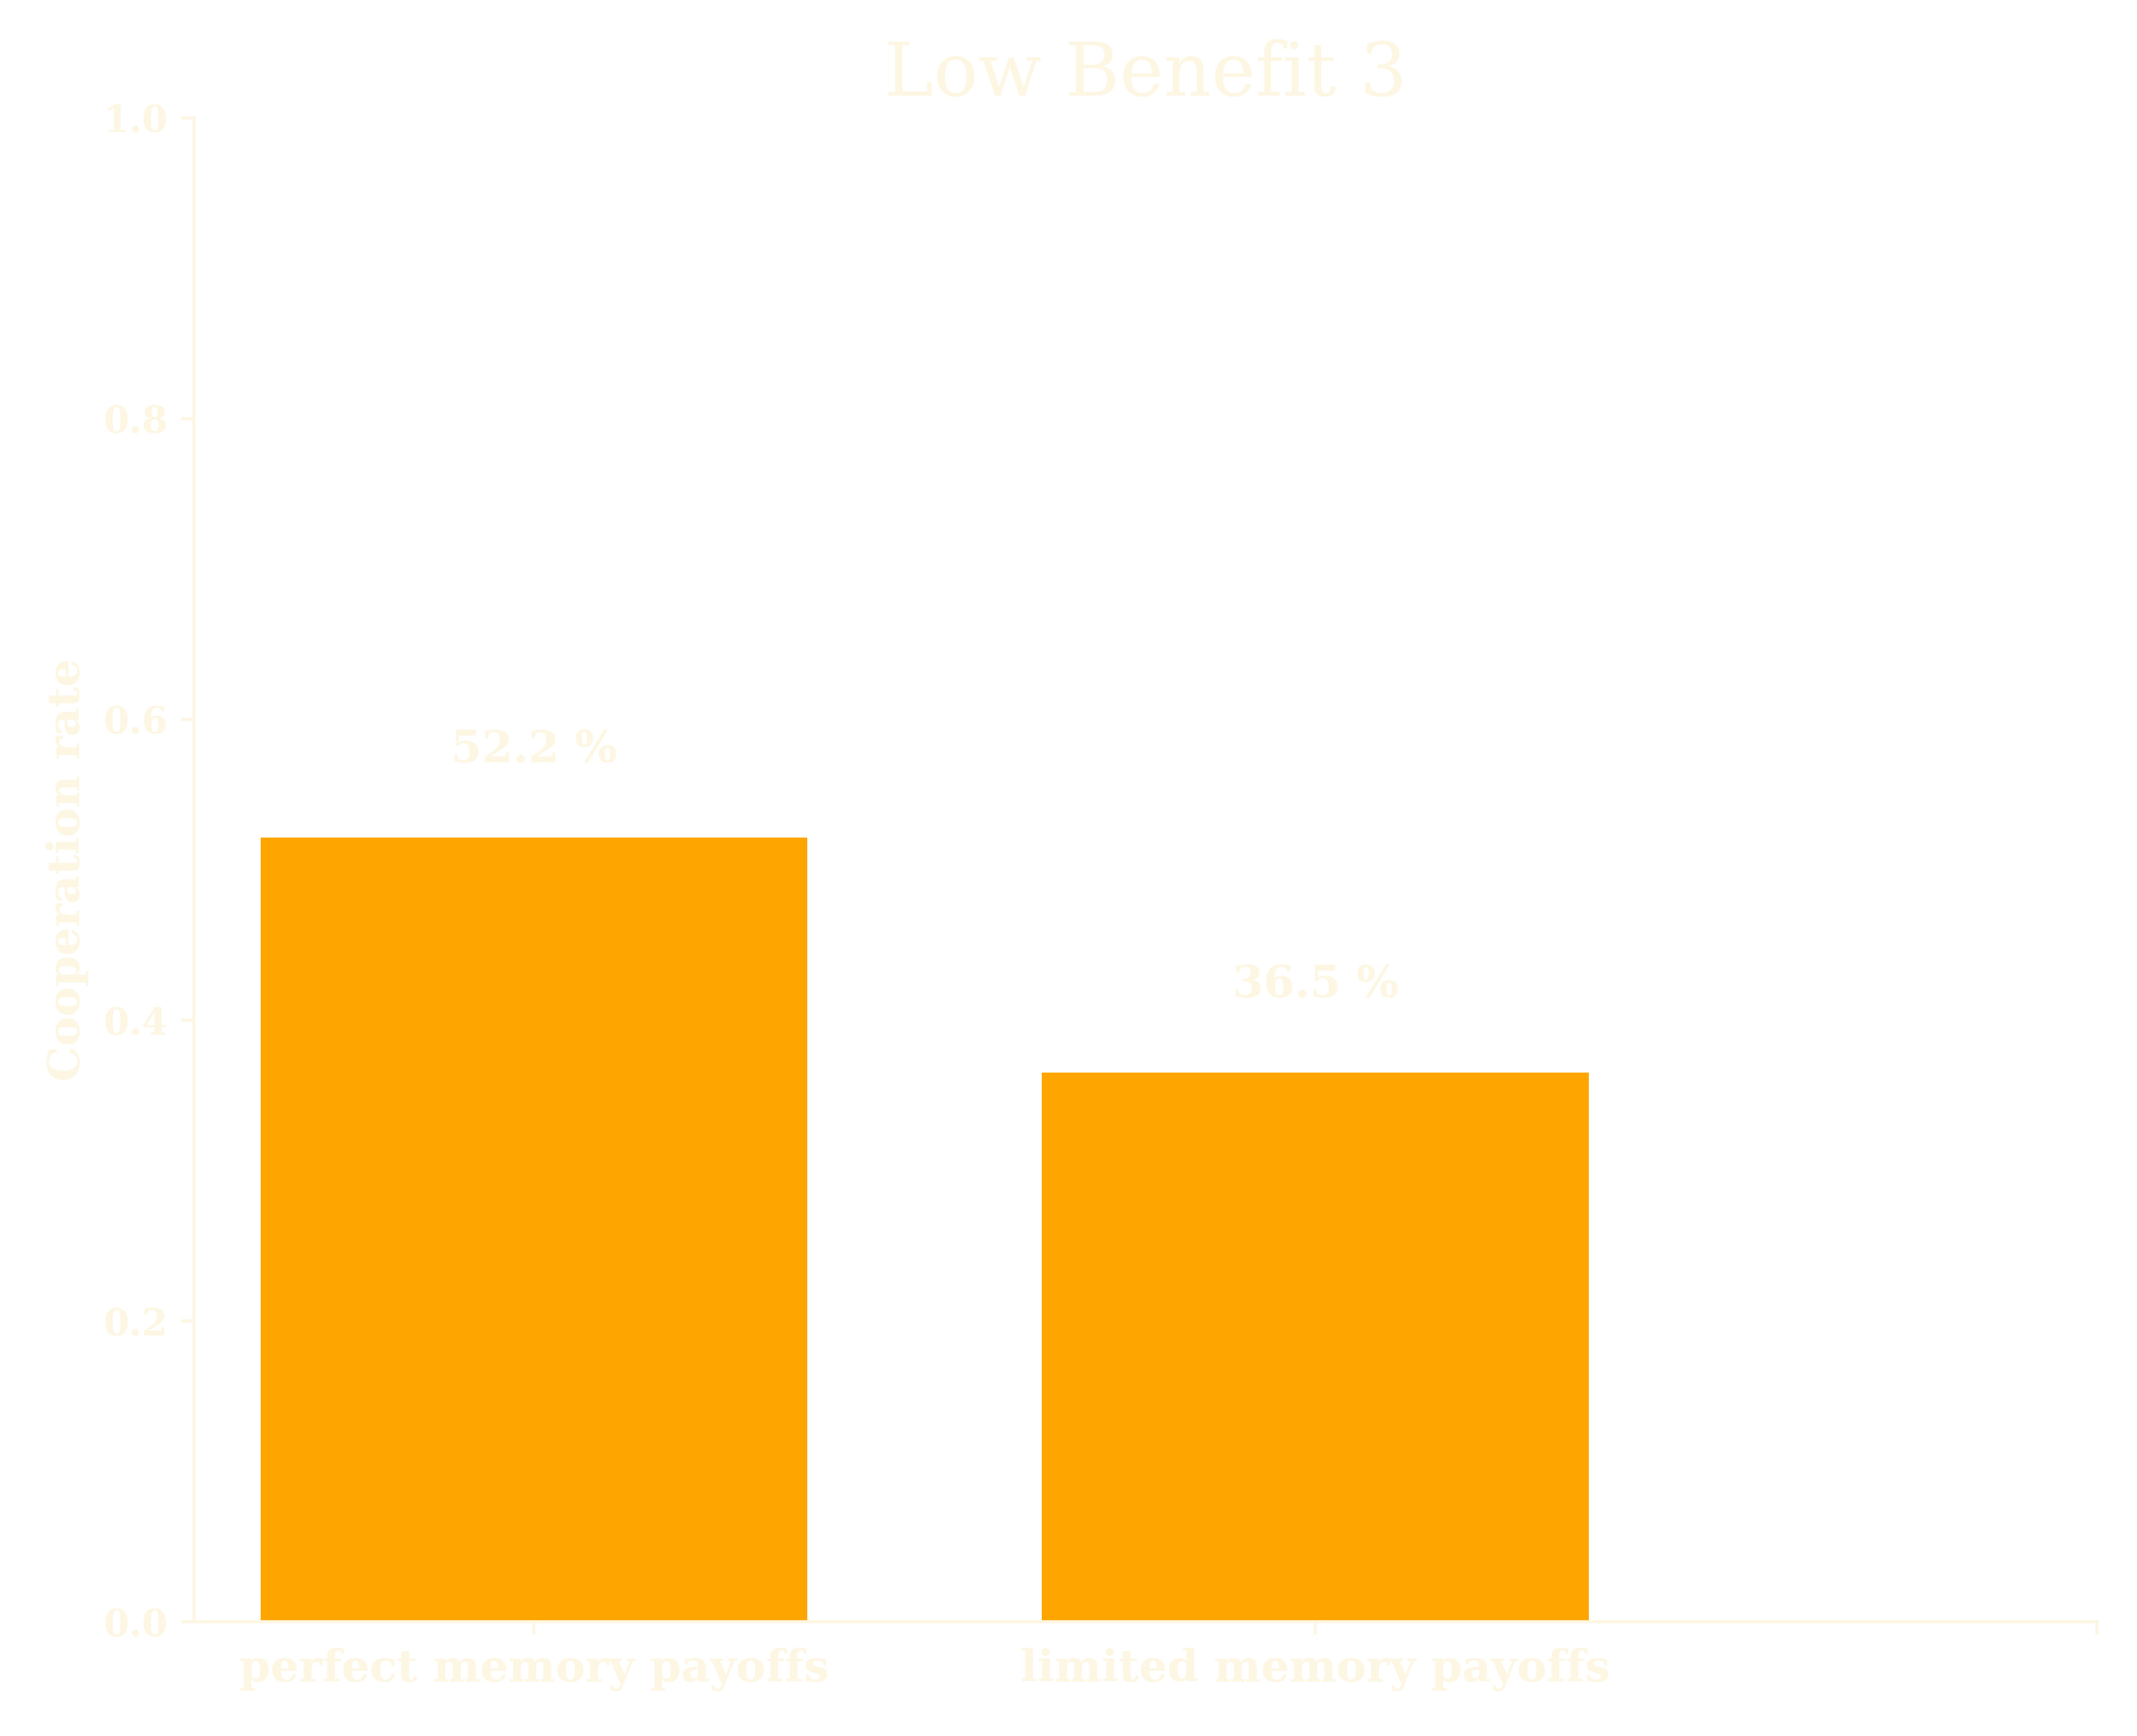
\includegraphics[width=.45\textwidth]{static/cooperation_b_3.png}
    \pause
    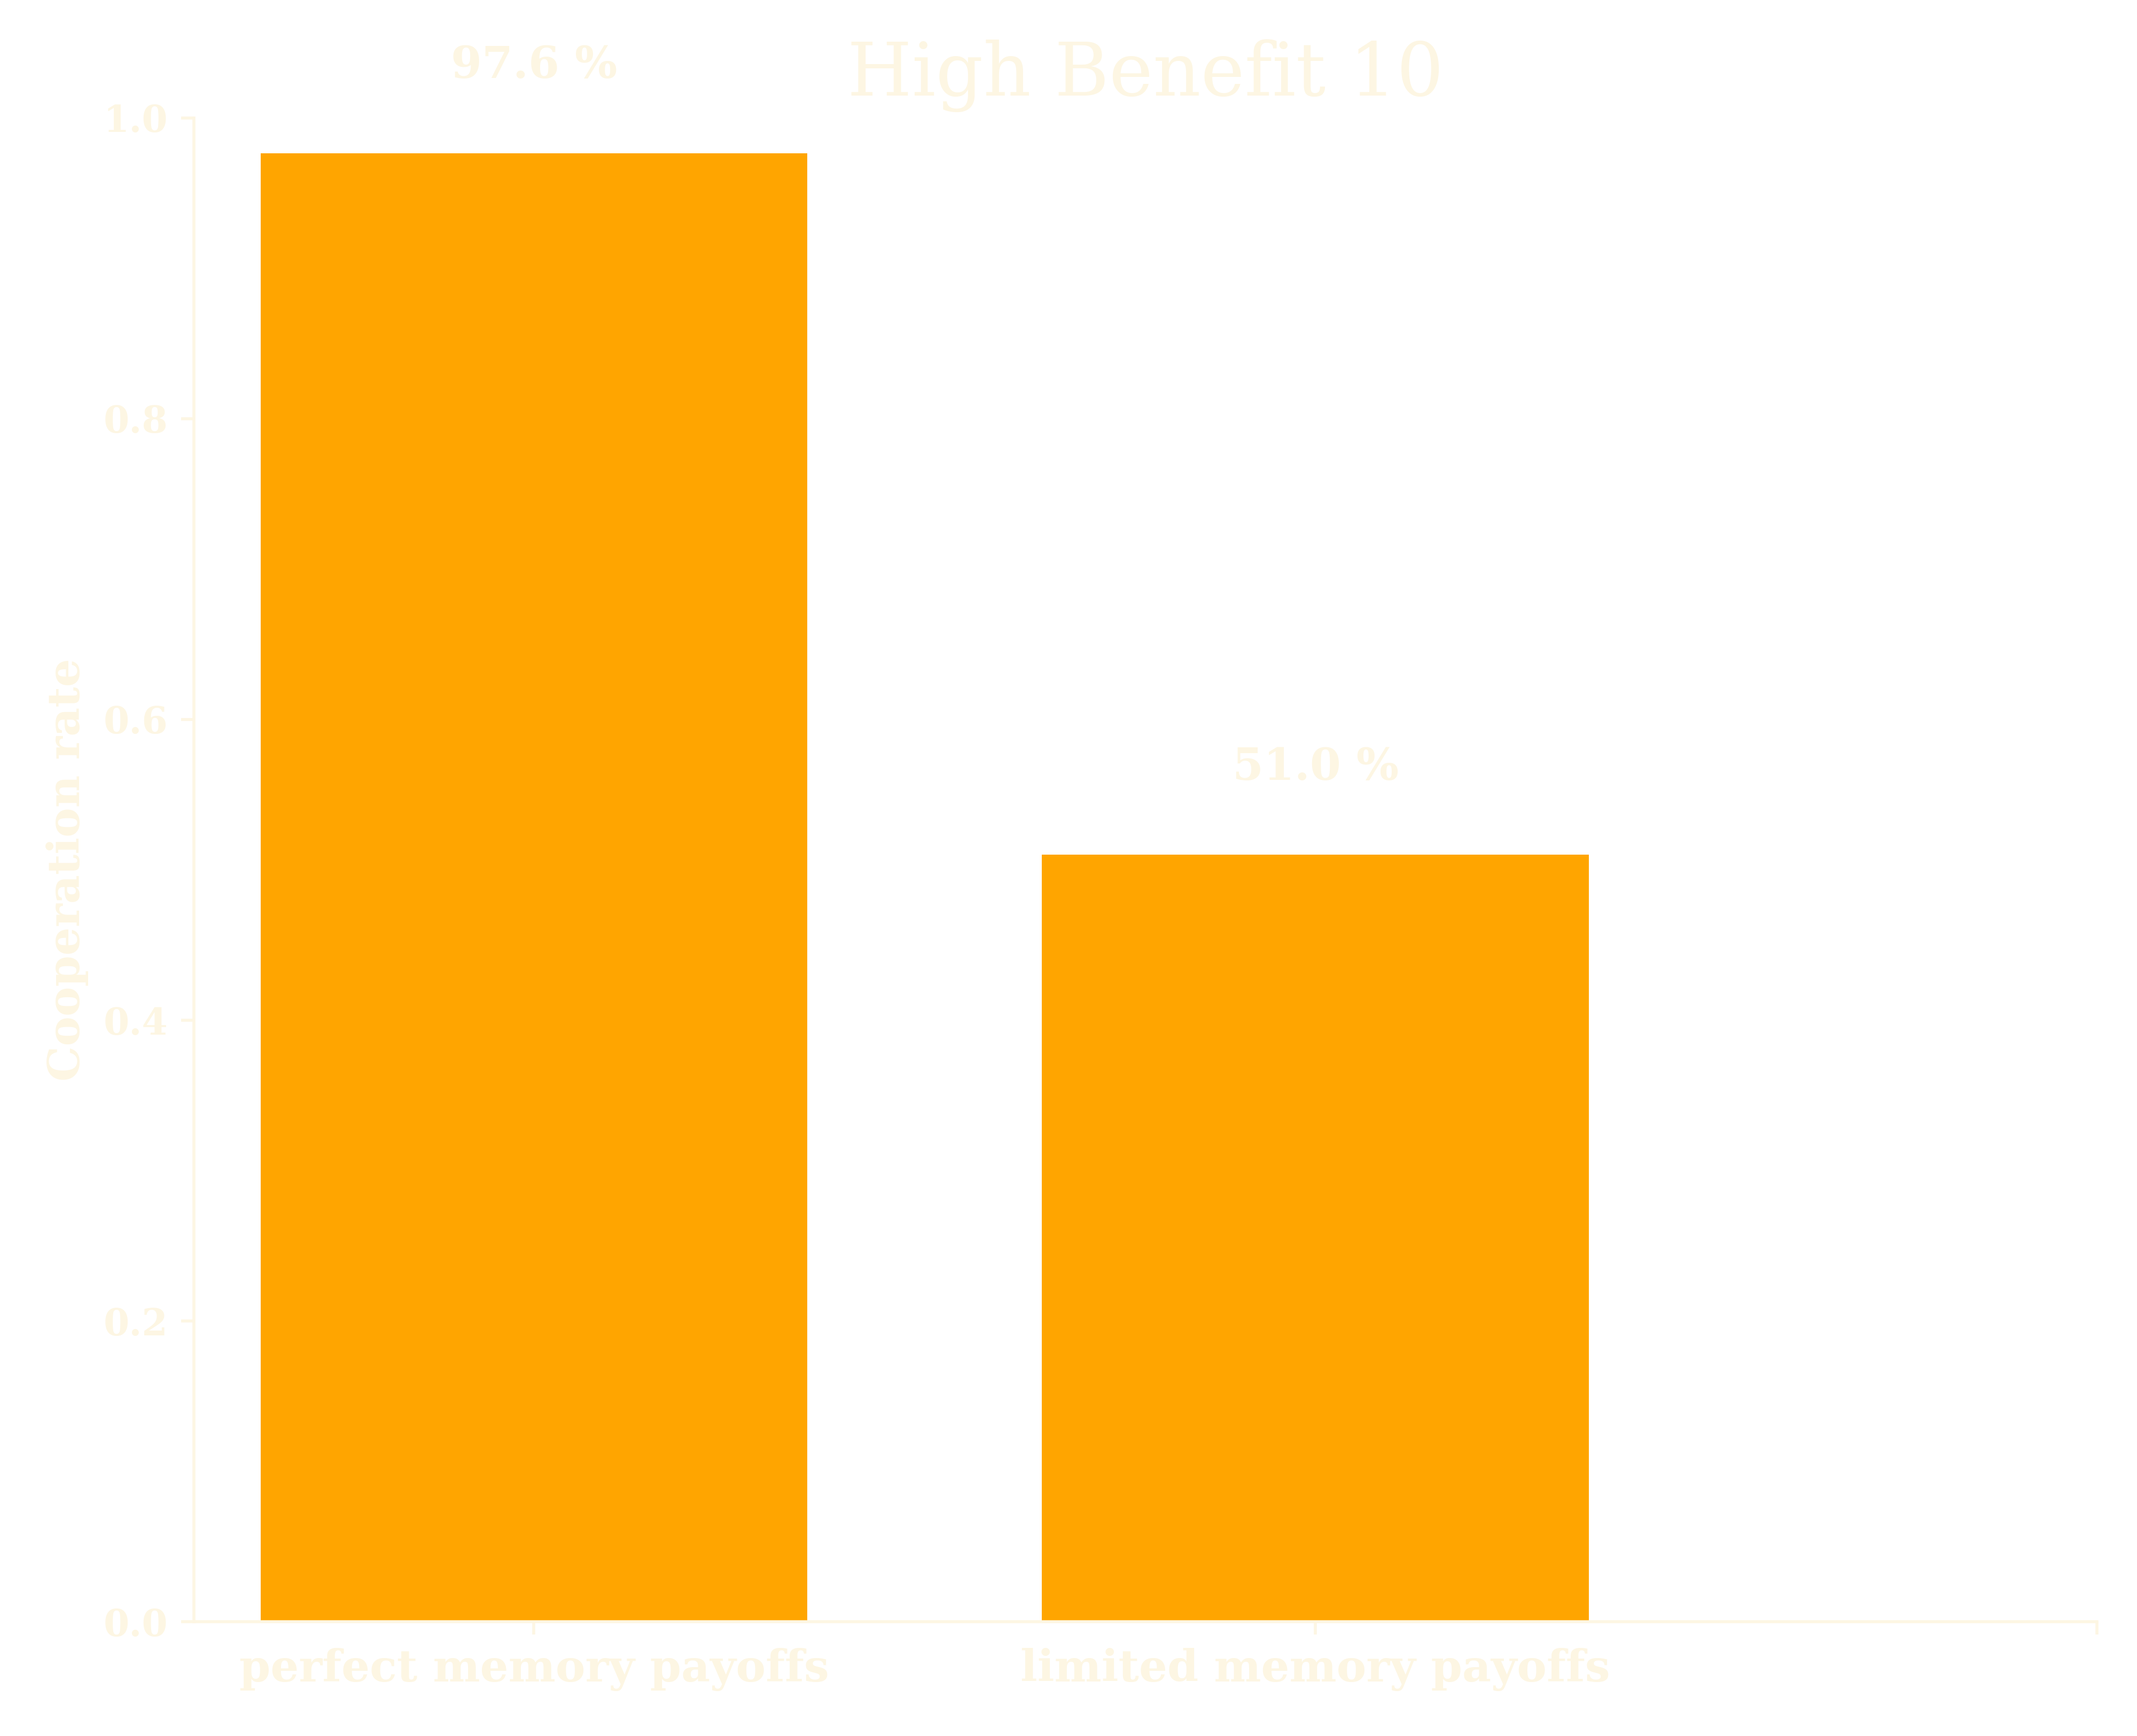
\includegraphics[width=.45\textwidth]{static/cooperation_b_10.png}
\end{frame}


\begin{frame}
    \centering
    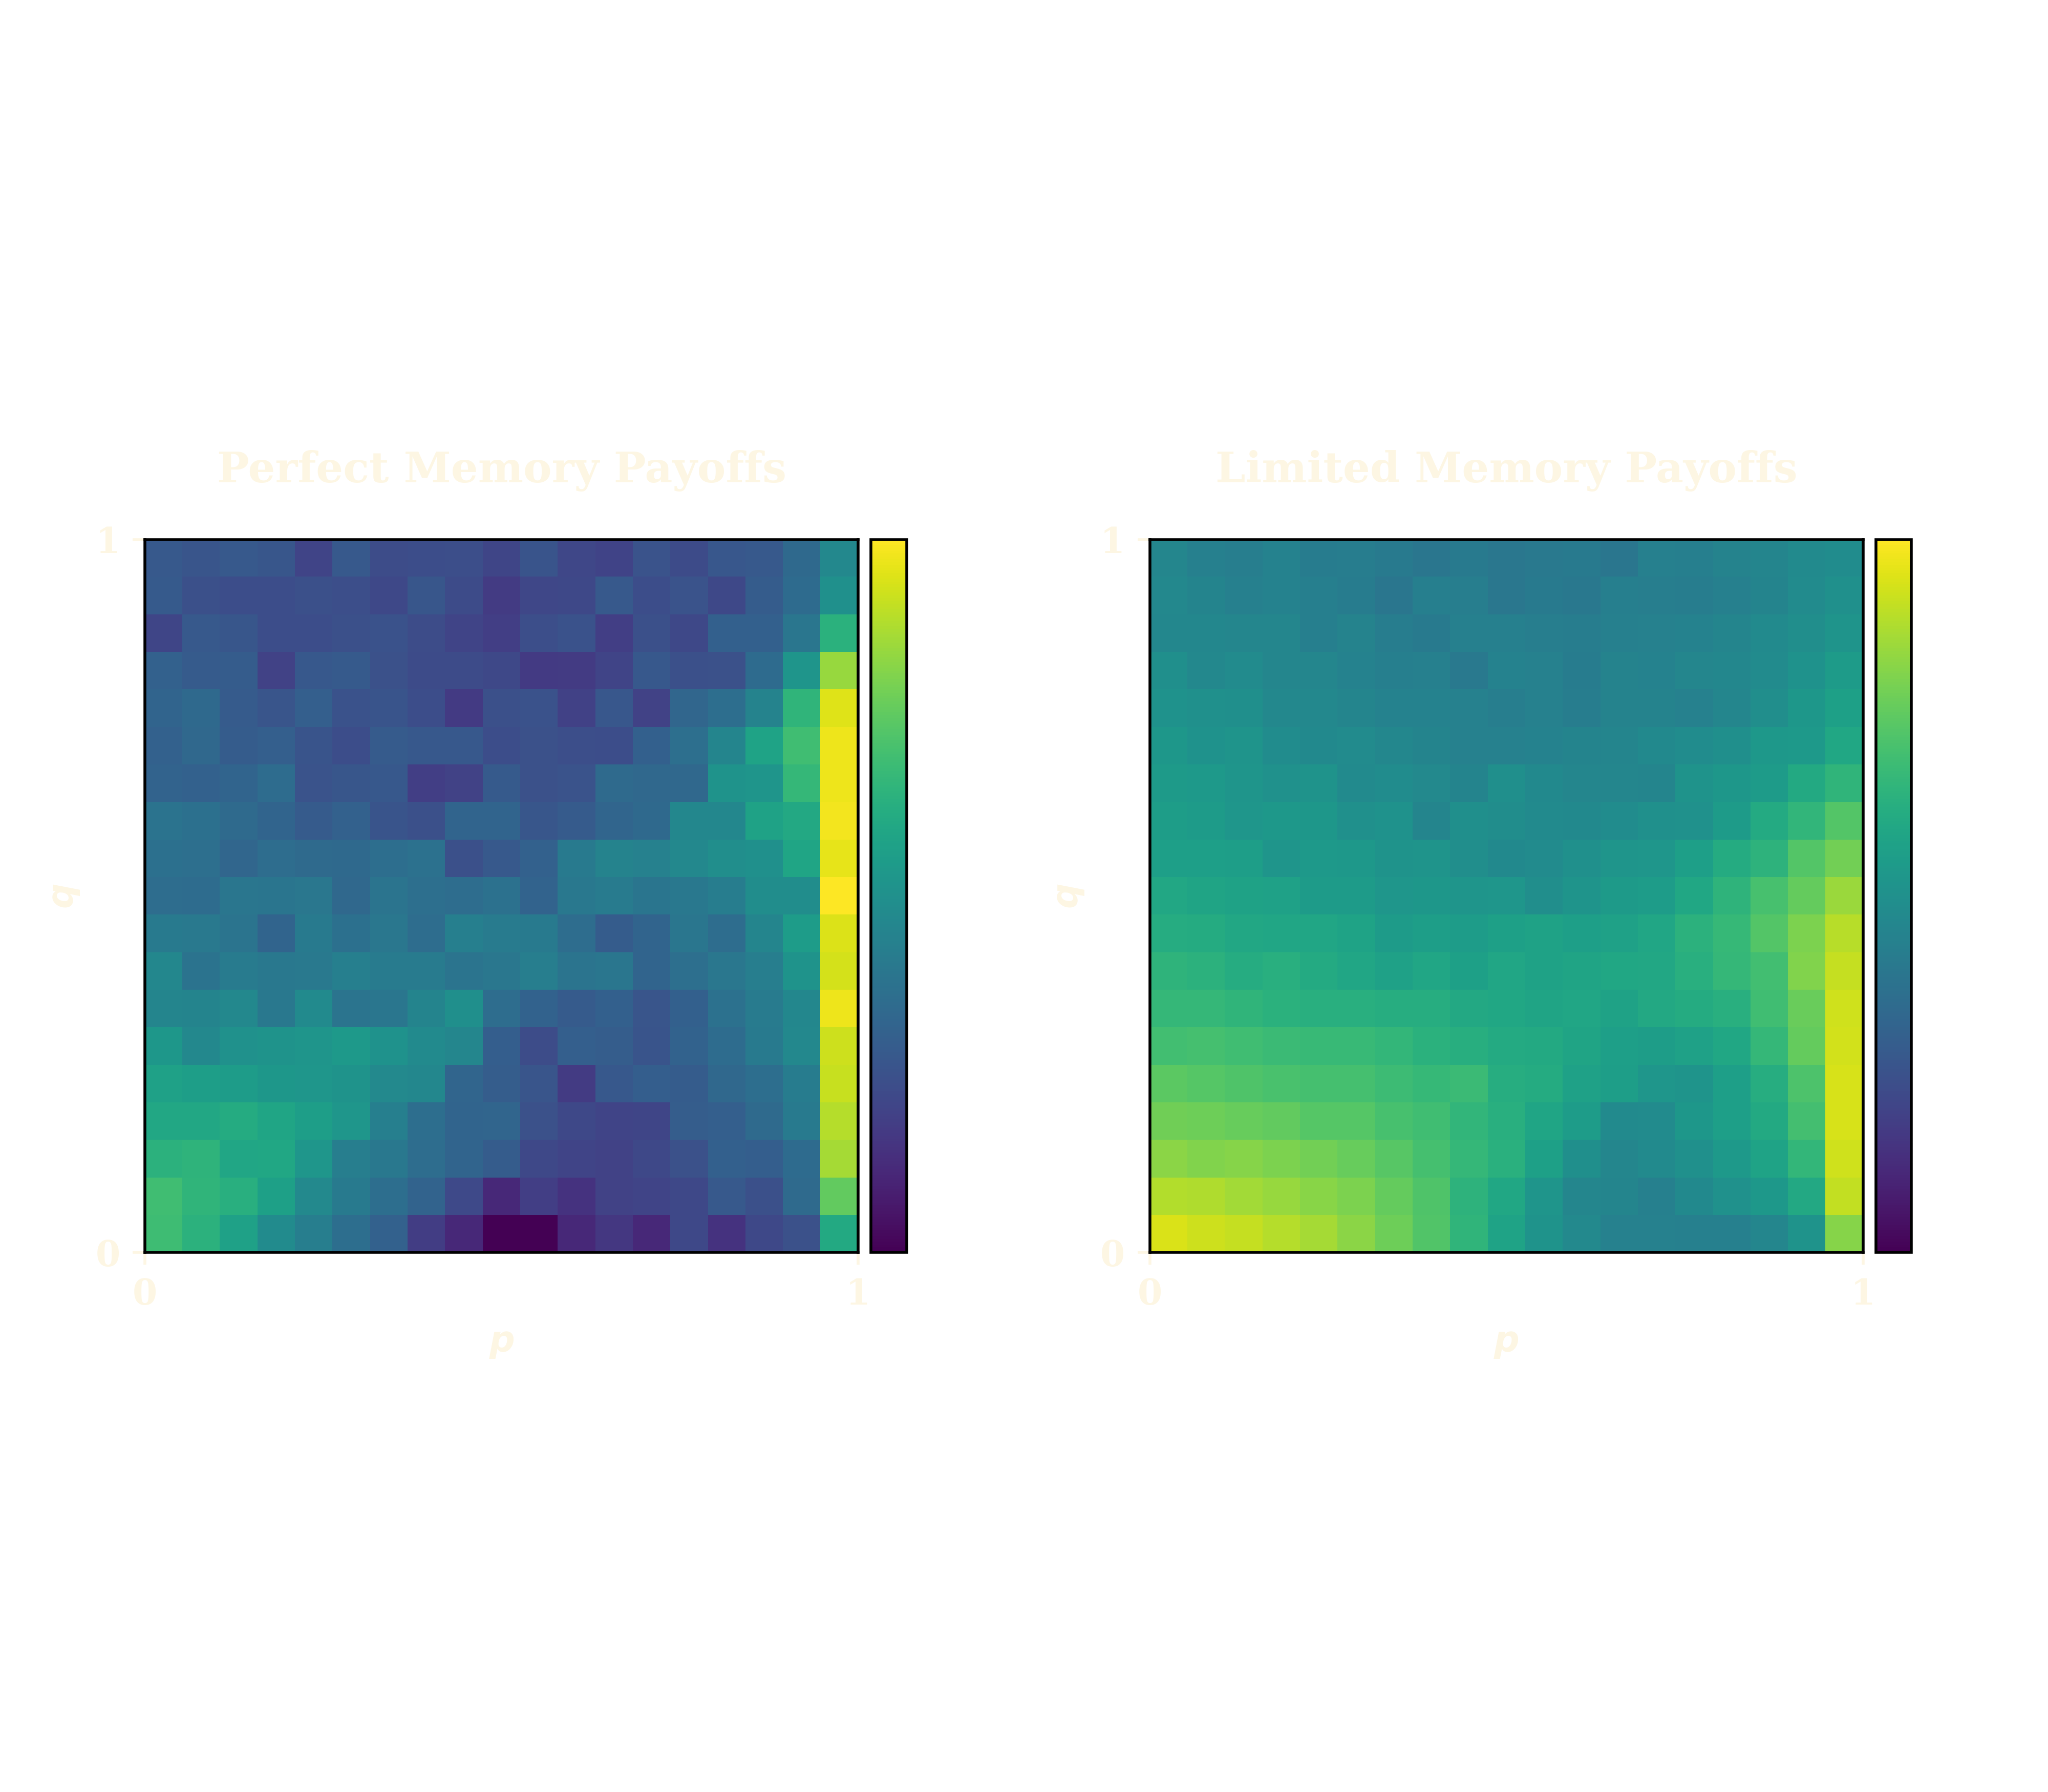
\includegraphics[width=.85\textwidth]{static/heatmap.png}
\end{frame}

\begin{frame}
    \centering
    \includestandalone[width=\textwidth]{static/more_memory}
\end{frame}

\begin{frame}
    \centering
    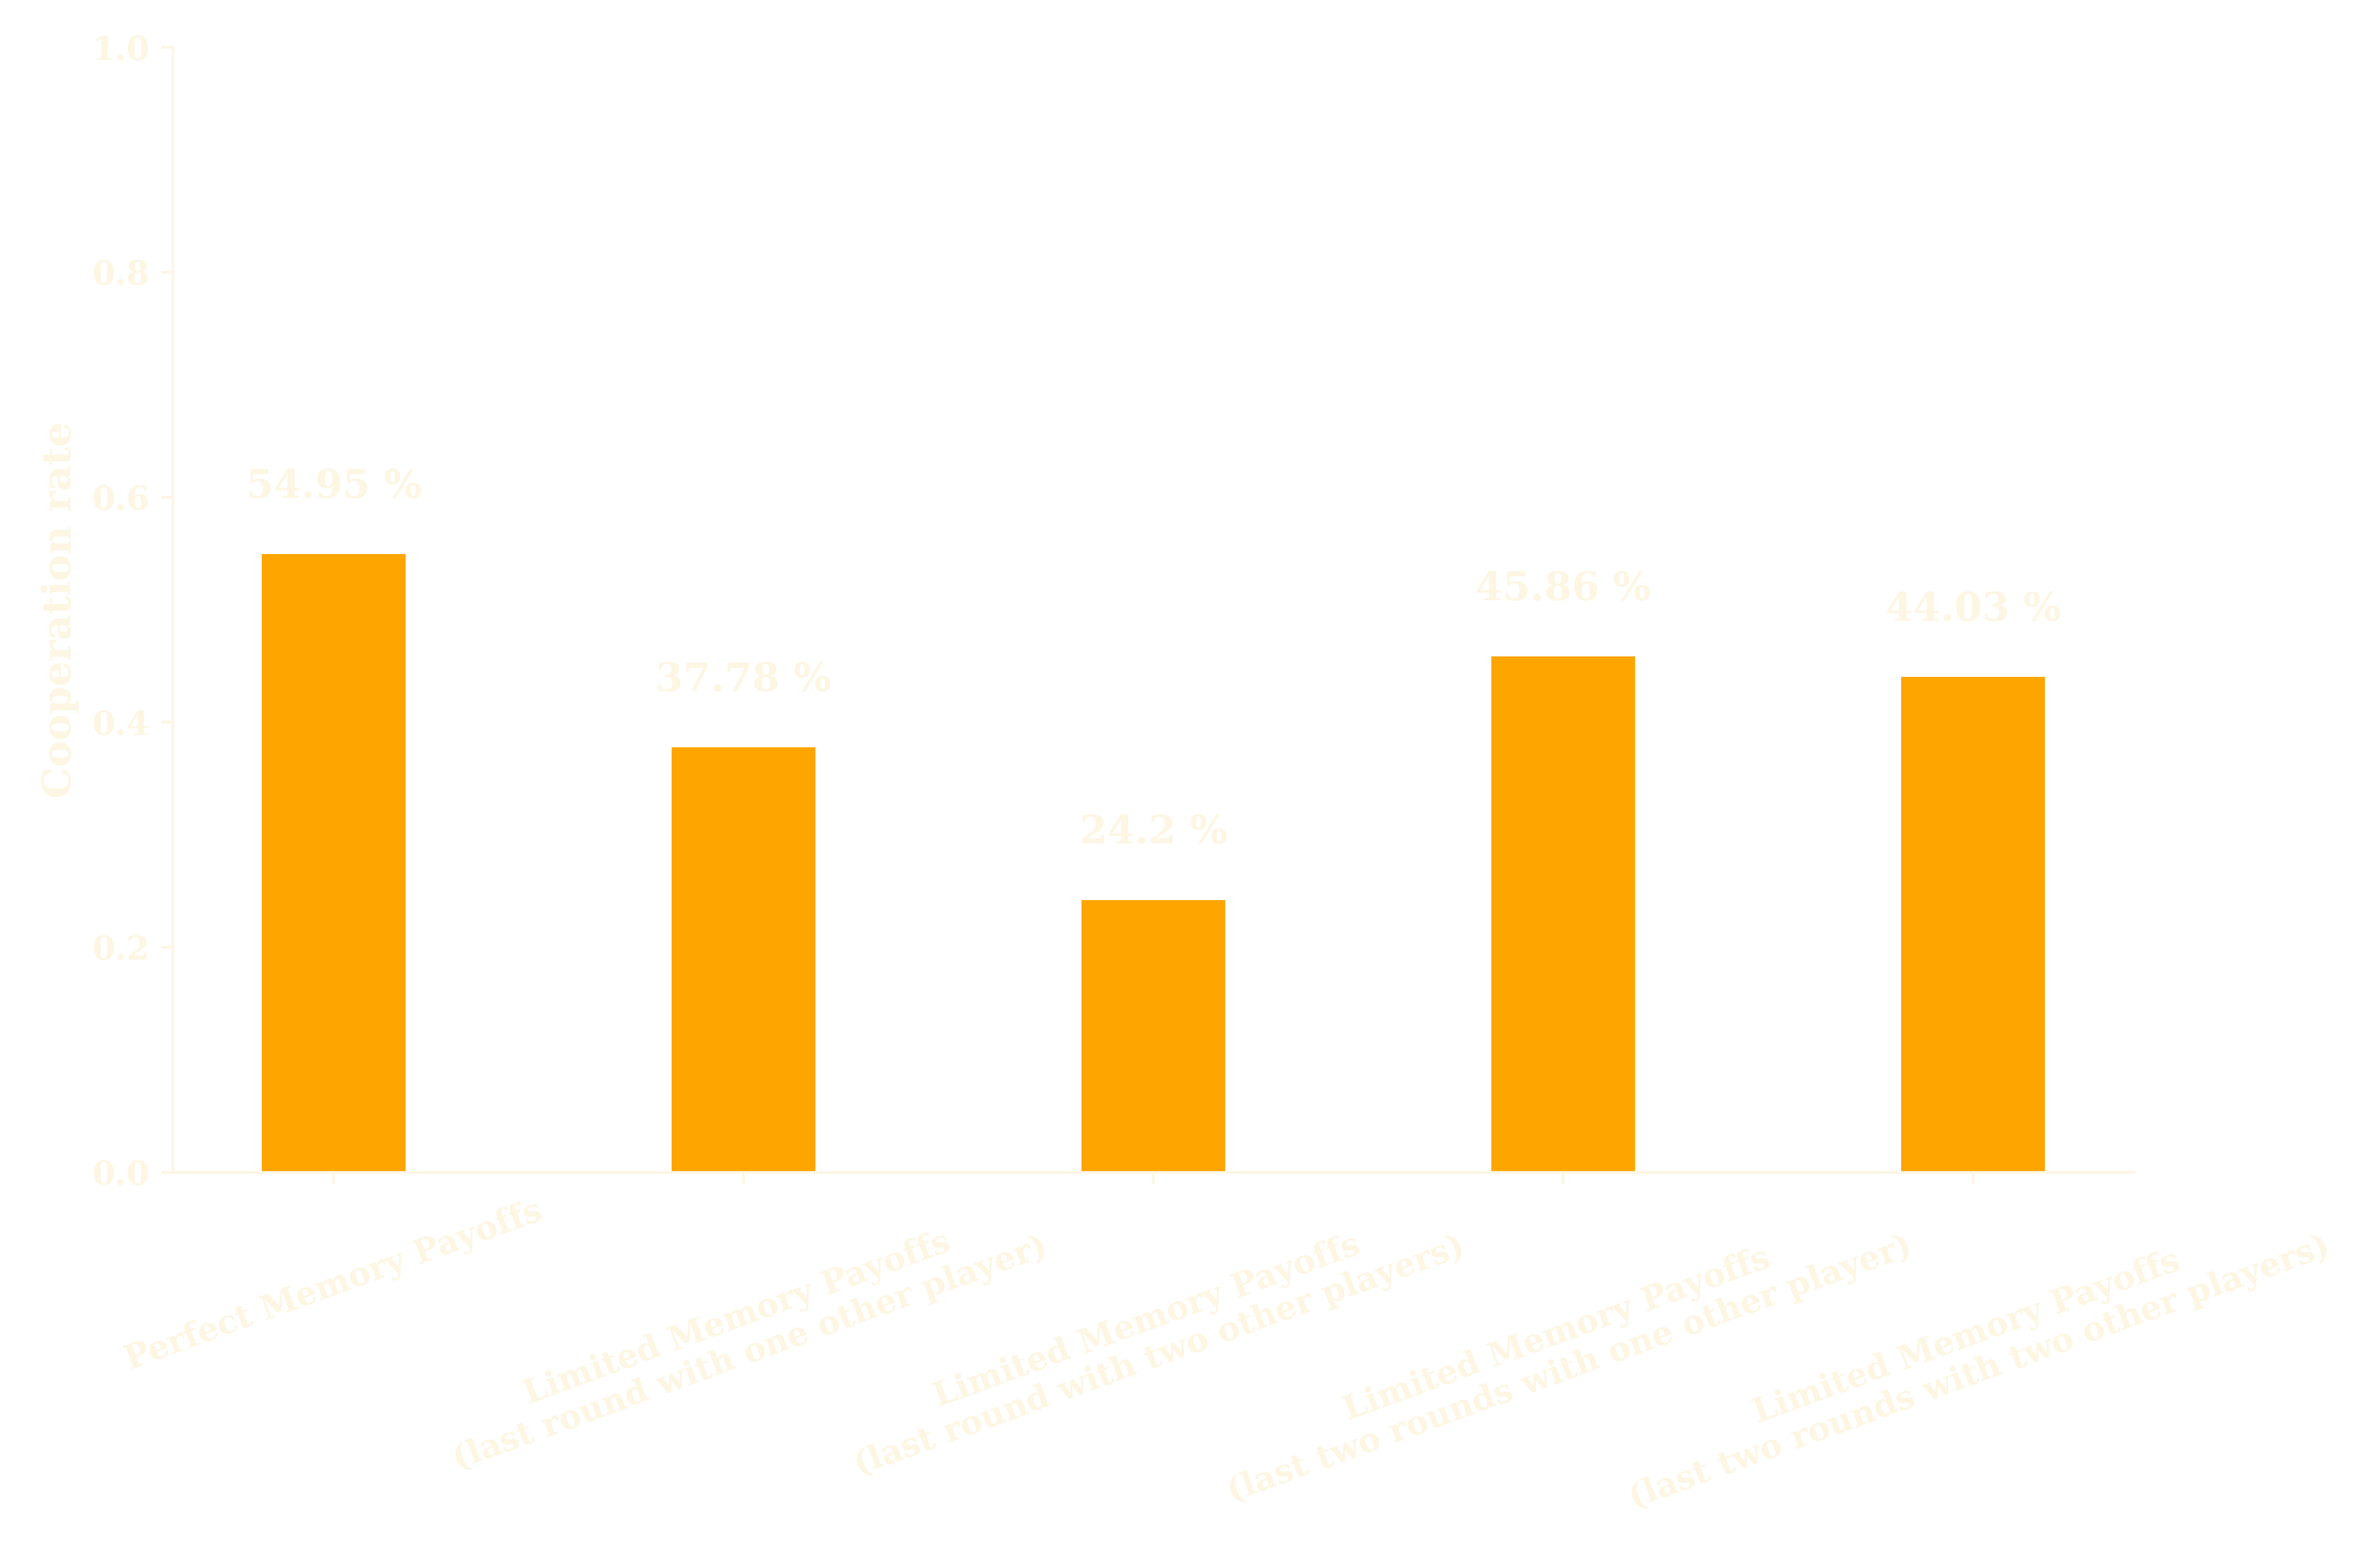
\includegraphics[width=\textwidth]{static/cooperation_rates.png}
\end{frame}

\begin{frame}
    \begin{center}
    \faTwitter \ @NikoletaGlyn \\
    \faTwitter \ @chilbe3 \\
    \end{center}
\end{frame}
\end{document}